\documentclass[11pt]{article}
\usepackage{hyperref}
\usepackage{xcolor}
\hypersetup{
    colorlinks=true,
    linkcolor=blue,
    filecolor=magenta,      
    urlcolor=red,
    pdftitle={Overleaf Example},
    pdfpagemode=FullScreen,
    }
\usepackage{amsmath,amssymb,amsfonts}
\usepackage{graphicx}

\setlength{\topmargin}{-.5in} \setlength{\textheight}{9.25in}
\setlength{\oddsidemargin}{0in} \setlength{\textwidth}{6.8in}

%%%%%%%%%%%%%%%%%%%%%%%%%%%%%%%%%%%%%%%%%%
\usepackage{pythonhighlight}
%%%%%%%%%%%%%%%%%%%%%%%%%%%
\newcounter{mycounter} 
\newcommand\showmycounter{\stepcounter{mycounter}\themycounter}
\usepackage{lipsum}
\newcommand\showlips{\stepcounter{mycounter}\lipsum[\value{mycounter}]}
%%%%%%%%%%%%%%%%%%%%%%%%%%%%%%%%%%%%%%
\usepackage{framed}
\usepackage{hyperref}
\usepackage{fancyhdr}

%%%%%%%%%%%%%%%%%%%%%%%%%%%%%%%%%%%%%%%%%%%%%%%%%%%%%%%%%%%%%
\usepackage{listings}
\usepackage{xcolor}

\definecolor{codegreen}{rgb}{0,0.6,0}
\definecolor{codegray}{rgb}{0.5,0.5,0.5}
\definecolor{codepurple}{rgb}{0.58,0,0.82}
\definecolor{backcolour}{rgb}{0.95,0.95,0.92}

\lstdefinestyle{mystyle}{
    backgroundcolor=\color{backcolour},   
    commentstyle=\color{codegreen},
    keywordstyle=\color{magenta},
    numberstyle=\tiny\color{codegray},
    stringstyle=\color{codepurple},
    basicstyle=\ttfamily\footnotesize,
    breakatwhitespace=false,         
    breaklines=true,                 
    captionpos=b,                    
    keepspaces=true,                 
    numbers=left,                    
    numbersep=5pt,                  
    showspaces=false,                
    showstringspaces=false,
    showtabs=false,                  
    tabsize=2
}

\lstset{style=mystyle}
%%%%%%%%%%%%%%%%%%%%%%%%%%%%%%%%%%%%%%%%%%%%%%%%%%%%%%%%%%%%%
\title{\LARGE VGU – CSE2022}
\author{\Huge Exercise 5 - Project (For Loop)}
\pagestyle{fancy}
\fancyhf{}
\lhead{\bfseries VGU}
\rhead{\bfseries  Programming 1}
\begin{document}

\maketitle


\begin{enumerate}

%1%%%%%%%%%%%%%%%%%%%%%%%%%%%%%%%%%%%%%%%%%%%%%%%%%%%%%%%%%%%%%%%%%%%%%%%%%%%%%%%%%%%%%%%%%%%%%%%%%%%%%%%%%%%%%%%%%%%%%%%%%%%%%%%%%%%%%%%%%%%%%%%%%%%%%%%%%%%%%%%%%%%%%%%%%%%%%%%%%%%%%%%
\item
\textbf{Implement these functions}

\begin{enumerate}
    \item Given a function f(x): $f(x) = x^{2} + 2x$ 
    \item Derivative of the function: $f'(x) = 2x + 2$
    \item Forward difference approximation: $f'(x) = \lim_{\Delta x\rightarrow 0}\frac{f(x+\Delta x) - f(x)}{\Delta x}$
    \item Central difference approximation: $f'(x) = \lim_{\Delta x\rightarrow 0}\frac{f(x+\frac{\Delta x}{2}) - f(x - \frac{\Delta x}{2})}{\Delta x}$
\end{enumerate}

%2%%%%%%%%%%%%%%%%%%%%%%%%%%%%%%%%%%%%%%%%%%%%%%%%%%%%%%%%%%%%%%%%%%%%%%%%%%%%%%%%%%%%%%%%%%%%%%%%%%%%%%%%%%%%%%%%%%%%%%%%%%%%%%%%%%%%%%%%%%%%%%%%%%%%%%%%%%%%%%%%%%%%%%%%%%%%%%%%%%%%%%%
\item 
\textbf{Write a function to performed background subtraction, as illustrated following}\\
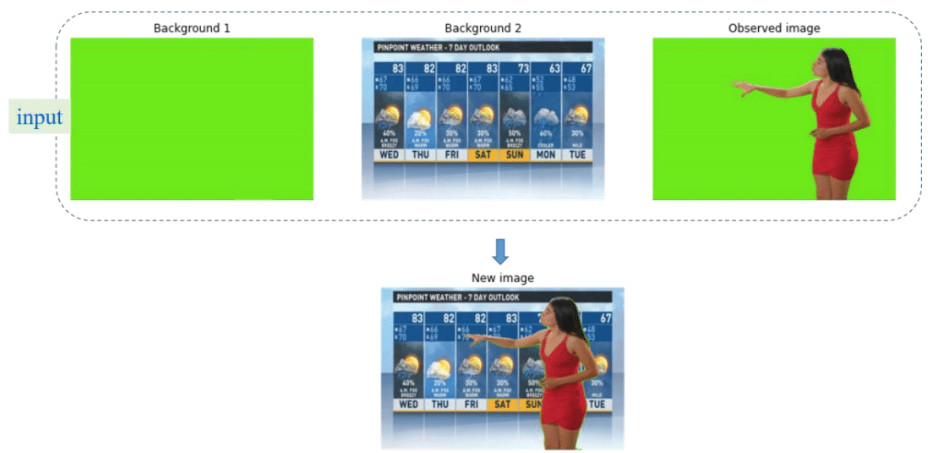
\includegraphics[width=\textwidth]{5-1}
    \begin{itemize}
        \item \textbf{Library to read an image:}\\
        \url{https://github.com/nothings/stb/blob/master/stb_image.h}
        \item \textbf{Library to write an image:}\\
        \url{https://github.com/nothings/stb/blob/master/stb_image_write.h} 
    \end{itemize}
\end{enumerate}
\end{document} 